\section{Modelo del dominio} % (fold)
\label{sec:modelo_del_dominio}
	{\it El Modelo de Dominio es una representación visual estática del entorno real objeto del proyecto.}

	Es decir, es {\bf una representación de las clases conceptuales del mundo real, no de componentes de software.} No se trata de un conjunto de diagramas que describen clases de software ni objetos de software con responsabilidades, sino más bien representa las clases conceptuales u objetos del mundo real en un dominio de interés. 

	El modelo de dominio  se debe concebir como un diccionario visual de abstracciones que será utilizado en fases posteriores y  cuya función principal es ayudar a comprender el problema a trata. Se dice que es una representación estática porque no representa la interacción en el tiempo de los objetos, sino que representa una visión \textit{parada} de las clases y sus interacciones. Incluye clases de objetos, asociaciones entre objetos y atributos de las clases de objeto.

	\subsection{Flujo del problema}
		Como ya se ha mencionado, existen dos actores principales, el médico y el paciente. 
		Un médico debe generar su horario de disponibilidad, en el que debe indicar, al menos, los días que trabaja, las horas que tiene disponible y el precio de la consulta. Por su parte, el paciente, puede ver los horarios de disponibilidad de distintos especialistas. Además, puede ver información asociada a cada médico y al centro en el que trabaja, tales como curriculum, localización, datos de contacto, etc.
		Una vez que el paciente tiene claro quién va a ser el especialista que lo visite, se asignará una hora en el horario del médico, y quedará concertada una cita. Por tanto, cada cita tendrá, al menos, una fecha, una hora, un médico y paciente.
		Toda la información de un paciente, tanto datos personales, como antecedentes médicos, resultados de diversas pruebas, diagnósticos, informes, etc, se almacena en la ficha médica. Por tanto, cada paciente tiene su única ficha. Un médico, por su parte, puede acceder a las fichas médicas de todos sus pacientes en cualquier momento.
		Con todos los datos sanitarios y con la cita concertada, médico y paciente acuden a la consulta. Ésta debe ser abonada por el paciente, generando la factura asociada, en la que aparecerán al menos, la fecha, el nombre del paciente y el coste. El resultado final de toda consulta suele ser un diagnóstico, que el médico genera y que debe ser además actualizado en la ficha médica del paciente, junto con el tratamiento establecido.

	\subsection{Diagrama del Modelo del Dominio}

	A continuación se muestra el modelo del dominio que representa el proyecto.
	\begin{figure}[H]
	  \centering
	    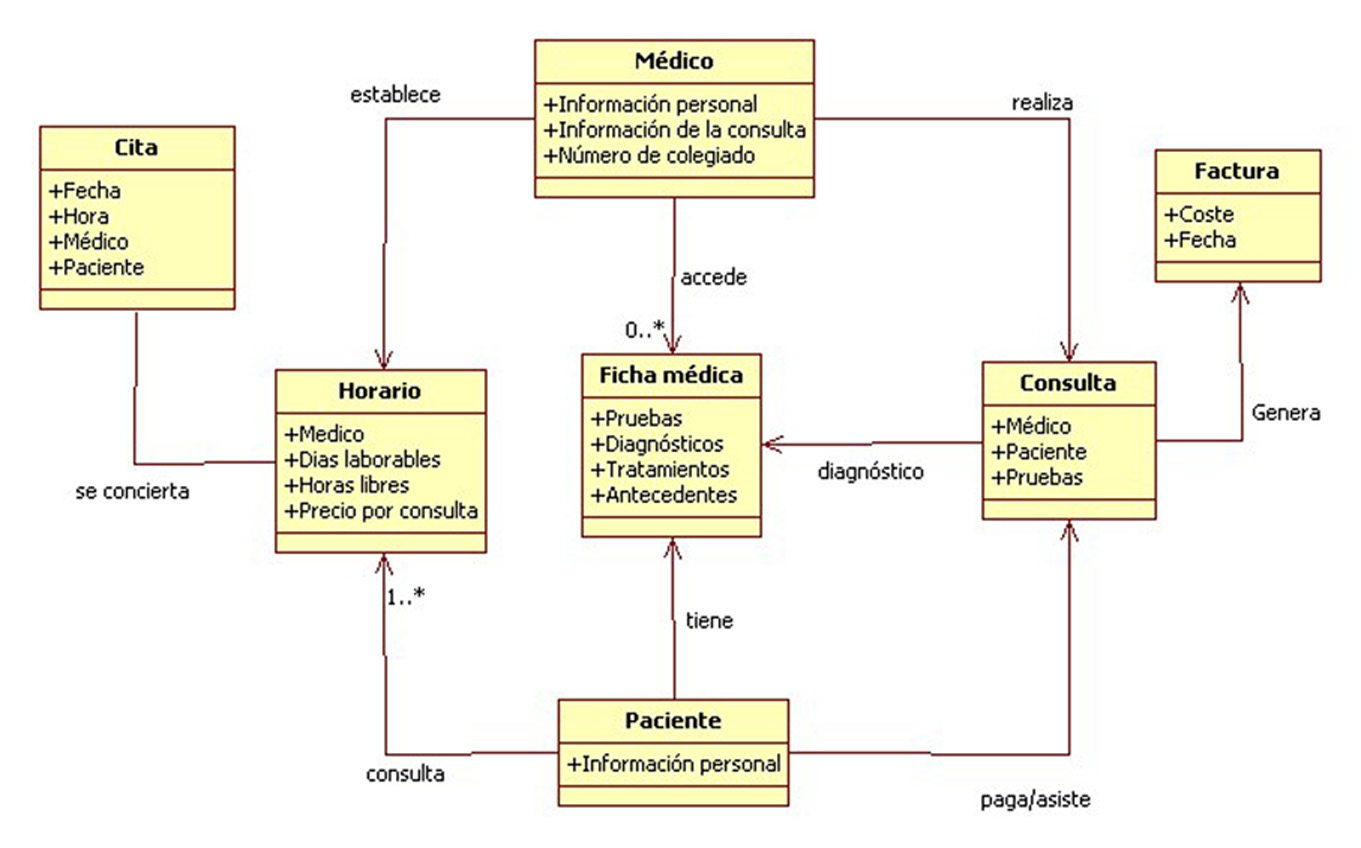
\includegraphics{img/modelo.jpg}
	  \caption{Modelo del dominio}
	  \label{modelodominio}
	\end{figure}

	\subsection{Glosario}
	Acorde a lo visto en la Figura \ref{modelodominio} vamos a establecer un pequeño glosario.

	\begin{itemize}
		\item \textbf{Cita.} Refleja que se concierta una consulta que supondrá el encuentro entre médico y paciente en la fecha y hora seleccionada. 
		\item \textbf{Consulta.} Encuentro entre médico y paciente.
		\item \textbf{Coste.} Transacción económica del importe de la consulta. 
		\item \textbf{Diagnóstico.} Calificación que da el médico a la enfermedad según los signos que advierte. Se añade a la ficha del paciente.
		\item \textbf{Factura.} Toda cita tiene un coste que debe ser abonado. Una vez realizado el pago, se genera una factura que corrobora que la transacción económica se ha producido.	
		\item \textbf{Ficha médica.} Información del paciente. Contiene tanto la información personal como todo tipo de información sanitaria: antecedentes, pruebas, diagnósticos, informes, tratamientos, etc.
		\item \textbf{Horario.} Horario del médico en el que aparece reflejado sus días laborables y sus horas disponibles, así como el coste de la consulta.
		\item \textbf{Médico.} Especialista encargado de la consulta con el paciente.
		\item \textbf{Paciente.} Persona con patología que acude a la consulta de un médico.
	\end{itemize}
% section modelo_del_dominio (end)